\documentclass[12pt,a4paper]{ctexart}

\usepackage[top=2.5cm,bottom=2.5cm,left=2cm,right=2cm]{geometry}
\usepackage{graphicx}
\usepackage[table]{xcolor}
\usepackage{booktabs}
\usepackage{multirow}
\usepackage{float}
\usepackage{hyperref}
\usepackage{tabularx}
\usepackage{array}
\usepackage{caption}
\usepackage{enumitem}
\usepackage{amssymb}

\definecolor{greenrate}{HTML}{C6EFCE}
\definecolor{yellowrate}{HTML}{FFEB9C}
\definecolor{redrate}{HTML}{FFC7CE}
\definecolor{headerbg}{HTML}{2F5496}
\definecolor{headerfg}{HTML}{FFFFFF}
\definecolor{grayrow}{HTML}{F2F2F2}

\graphicspath{{images/}}

\hypersetup{colorlinks=true,linkcolor=blue,urlcolor=blue}
\setlength{\tabcolsep}{5pt}

\title{\textbf{阶段性学情分析（2026 年 7 月）}}
\author{2026-07-31}
\date{}

\begin{document}
\maketitle
\thispagestyle{empty}
\newpage
\tableofcontents
\newpage

% ============================================================
\section{本月概况}
% ============================================================

\begin{enumerate}[leftmargin=*,itemsep=6pt]
    \item \textbf{三条主线}

    7 月完成了三件事：\textbf{408 一刷收官}（计网 7/1--7/5 完成最后 150 题，四科 2437 题全部刷完）；\textbf{数学强化推进}（严选题第 3--7 章 + 880 选填/解答共 423 题）；\textbf{英语阅读推进}（完成 2017--2019 年真题阅读 11 篇）。全月合计完成 \textbf{628 题}、正确 487 题，综合正确率 \textbf{77.5\%}。

    \item \textbf{节奏：中旬休息一周，月底逐步恢复}

    7 月上旬（1--18 日）保持了较高强度；\textbf{13 号之后开始休息}，数据上空窗约一周（7/19--7/26 基本无记录）；7/27 从严选题第七章（无穷级数）重新启动，7/28--7/31 数学与英语都恢复了推进，到今天（8 月初）才渐渐回到正常学习节奏。

    \item \textbf{恢复情况可以从英语阅读直接看出来}

    休息前 9 篇阅读平均用时 \textbf{15.2 分钟}、正确率 \textbf{80\%}；休整一周后 7/30 做的 2019 Text2 正确率掉到 \textbf{40\%}、用时 \textbf{20 分钟}（7 月最慢），明显生疏；7/31 的 2019 Text3 就回到 \textbf{100\%、14 分钟}——一周的空窗会让手感短期下降，但底子还在，恢复很快。

\end{enumerate}

\section{7 月完成量一览}

\begin{table}[H]
\centering
\begin{tabular}{lrrrr}
\hline
\rowcolor{headerbg}\textcolor{headerfg}{\textbf{板块}} & \textcolor{headerfg}{\textbf{内容}} & \textcolor{headerfg}{\textbf{题量}} & \textcolor{headerfg}{\textbf{正确}} & \textcolor{headerfg}{\textbf{正确率}} \\
数学·严选题 & 第 3--7 章（7/2--7/27） & 233 & 172 & \cellcolor{yellowrate}73.8\% \\
数学·880   & 选填 2 章 + 解答 2 章（7/4、7/29） & 190 & 147 & \cellcolor{yellowrate}77.4\% \\
408·计网   & 第 5--6 章收官（7/1--7/5） & 150 & 125 & \cellcolor{greenrate}83.3\% \\
英语·阅读  & 2017--2019 完成 11 篇（7/4--7/31） & 55 & 43 & \cellcolor{yellowrate}78.2\% \\
\rowcolor{grayrow}\textbf{合计} & & \textbf{628} & \textbf{487} & \textbf{77.5\%} \\
\hline
\end{tabular}
\caption{7 月各板块完成情况（英语按实际完成的 55 题计，2019 Text4 未做）}
\end{table}

\begin{figure}[H]
\centering
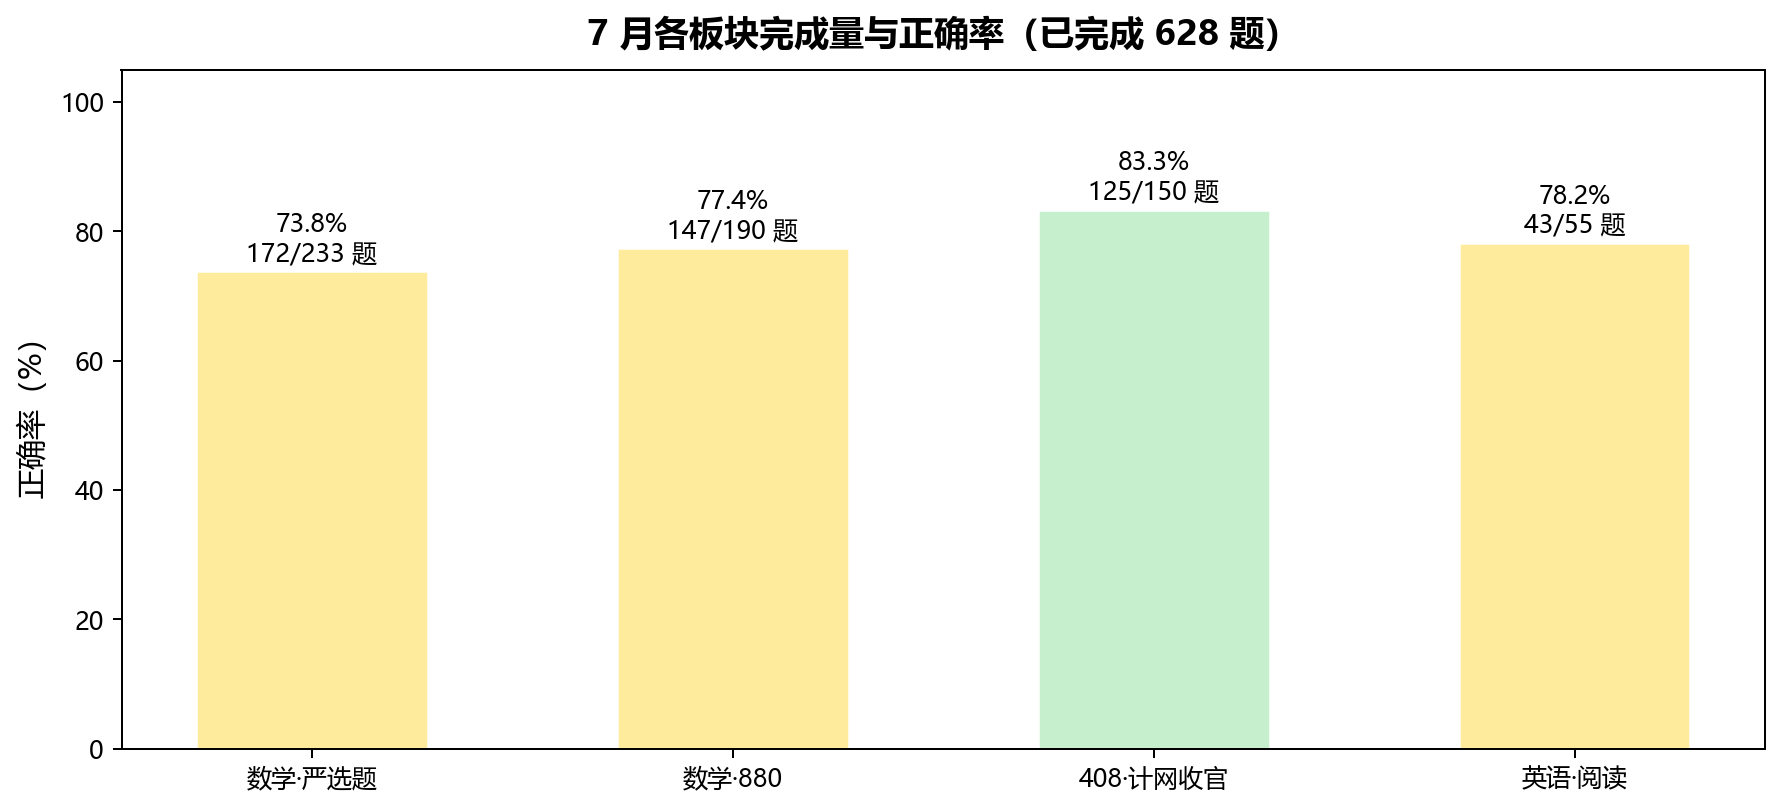
\includegraphics[width=0.82\textwidth]{july_workload.png}
\caption{7 月各板块完成量与正确率}
\end{figure}

\newpage

% ============================================================
\section{数学}
% ============================================================

\subsection{武忠祥严选题（7 月完成第 3--7 章）}

\begin{table}[H]
\footnotesize
\centering
\begin{tabular}{lrrrrrrrr}
\hline
\rowcolor{headerbg}\textcolor{headerfg}{\textbf{章节}} & \textcolor{headerfg}{\textbf{日期}} & \textcolor{headerfg}{\textbf{选择}} & \textcolor{headerfg}{\textbf{填空}} & \textcolor{headerfg}{\textbf{问答}} & \textcolor{headerfg}{\textbf{合计}} & \textcolor{headerfg}{\textbf{正确率}} & \\
第三章 一元函数积分学 & 7/2 & 11/13 & 18/24 & 13/25 & 42/62 & \cellcolor{redrate}67.7\% & \\
第四章 常微分方程 & 7/11 & 7/7 & 8/8 & 13/19 & 28/34 & \cellcolor{greenrate}82.4\% & \\
第五章 多元函数微分学 & 7/16 & 13/16 & 8/12 & 17/22 & 38/50 & \cellcolor{yellowrate}76.0\% & \\
第六章 二重积分 & 7/18 & 12/12 & 8/10 & 13/18 & 33/40 & \cellcolor{greenrate}82.5\% & \\
第七章 无穷级数 & 7/27 & 12/17 & 3/7 & 16/23 & 31/47 & \cellcolor{redrate}66.0\% & \\
\rowcolor{grayrow}7 月小计 & & 55/65 & 45/61 & 72/107 & 172/233 & 73.8\% & \\
\hline
\end{tabular}
\caption{严选题 7 月推进明细（正确数/总题数）}
\end{table}

\begin{itemize}
\item 严选题累计（第 1--7 章）：\textbf{336 题 / 254 对 / 75.6\%}（选择 83.0\%、填空 78.8\%、问答 69.2\%）；第 8、9 章（数一专属）尚未开始。
\item 失分点集中在\textbf{填空与问答}：7 月填空 73.8\%、问答 67.3\%。第七章无穷级数是恢复后第一天做的（7/27），填空仅 3/7（42.9\%），也是全月最低的一章。
\end{itemize}

\subsection{李林 880（7 月）}

\begin{table}[H]
\footnotesize
\centering
\begin{tabular}{lrrrr}
\hline
\rowcolor{headerbg}\textcolor{headerfg}{\textbf{区块}} & \textcolor{headerfg}{\textbf{章节}} & \textcolor{headerfg}{\textbf{日期}} & \textcolor{headerfg}{\textbf{题量}} & \textcolor{headerfg}{\textbf{正确率}} \\
选填 & 第三章 一元函数积分学及其应用 & 7/4 & 65 & \cellcolor{greenrate}84.6\% \\
选填 & 第八章 无穷级数 & 7/29 & 35 & \cellcolor{greenrate}80.0\% \\
解答 & 第三章（综合篇三个物理应用未做） & 7/4 & 58 & \cellcolor{redrate}69.0\% \\
解答 & 第八章 无穷级数 & 7/29 & 32 & \cellcolor{yellowrate}75.0\% \\
\rowcolor{grayrow}7 月小计 & 选填 100/83（83.0\%） + 解答 90/64（71.1\%） & & 190 & 77.4\% \\
\hline
\end{tabular}
\caption{880 7 月推进明细}
\end{table}

\begin{itemize}
\item 第五章多元函数微分学 7/28 开始（题量未统计）；空间解析几何内容未完成。
\item 880 累计：选填 \textbf{206/177（85.9\%）}、解答 \textbf{147/99（67.3\%）}、合计 \textbf{353/276（78.2\%）}；线性代数、概率论未开始。
\item 张宇 1000 题 7 月无推进（基础篇 257/203=79.0\% 已于 5 月完成，强化/综合篇未开始）。
\end{itemize}

\begin{figure}[H]
\centering
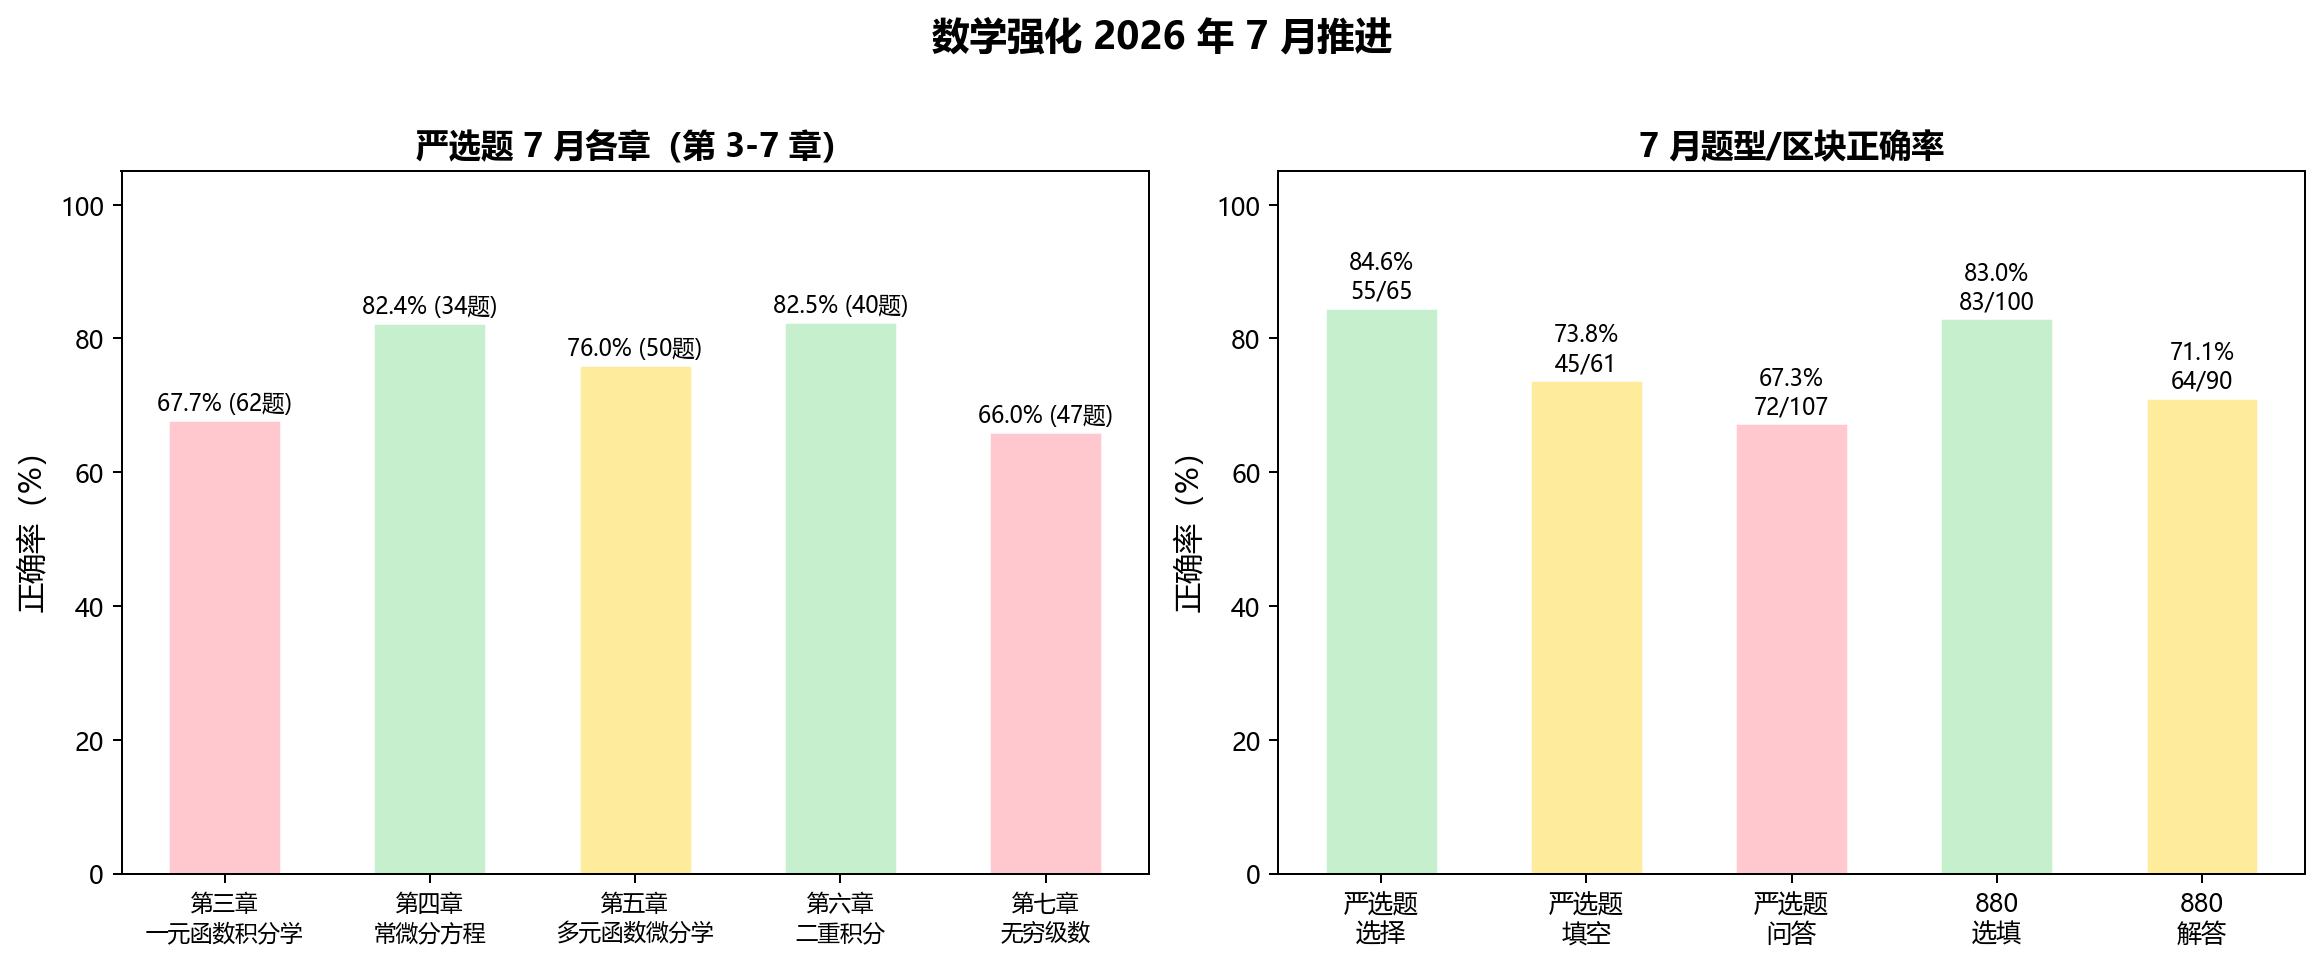
\includegraphics[width=0.95\textwidth]{july_math_progress.png}
\caption{数学强化 7 月推进：严选题各章与题型正确率}
\end{figure}

\newpage

% ============================================================
\section{408 计算机统考}
% ============================================================

\subsection{计网一刷收官（7/1--7/5）}

\begin{table}[H]
\footnotesize
\centering
\begin{tabular}{lrrrr}
\hline
\rowcolor{headerbg}\textcolor{headerfg}{\textbf{小节}} & \textcolor{headerfg}{\textbf{日期}} & \textcolor{headerfg}{\textbf{题量}} & \textcolor{headerfg}{\textbf{正确}} & \textcolor{headerfg}{\textbf{正确率}} \\
5.1 传输层提供的服务 & 7/1 & 10 & 9 & \cellcolor{greenrate}90.0\% \\
5.2 UDP & 7/1 & 17 & 11 & \cellcolor{redrate}64.7\% \\
5.3 TCP & 7/3 & 61 & 51 & \cellcolor{greenrate}83.6\% \\
6.1 网络应用模型 & 7/4 & 6 & 6 & 100\% \\
6.2 域名系统 & 7/4 & 14 & 11 & \cellcolor{yellowrate}78.6\% \\
6.3 文件传输协议 & 7/4 & 11 & 10 & \cellcolor{greenrate}90.9\% \\
6.4 电子邮件 & 7/5 & 12 & 12 & 100\% \\
6.5 万维网 & 7/5 & 19 & 15 & \cellcolor{yellowrate}78.9\% \\
\rowcolor{grayrow}合计（传输层 80.7\% / 应用层 87.1\%） & & 150 & 125 & \cellcolor{greenrate}83.3\% \\
\hline
\end{tabular}
\caption{计网 7 月收官明细}
\end{table}

\subsection{四科一刷终态}

\begin{table}[H]
\centering
\begin{tabular}{lrrrr}
\hline
\rowcolor{headerbg}\textcolor{headerfg}{\textbf{科目}} & \textcolor{headerfg}{\textbf{题量}} & \textcolor{headerfg}{\textbf{正确}} & \textcolor{headerfg}{\textbf{正确率}} & \textcolor{headerfg}{\textbf{状态}} \\
数据结构 & 634 & 538 & \cellcolor{greenrate}84.9\% & 一刷完成 \\
计算机网络 & 561 & 457 & \cellcolor{greenrate}81.5\% & 一刷完成（7/5） \\
操作系统 & 650 & 484 & \cellcolor{yellowrate}74.5\% & 一刷完成 \\
计算机组成原理 & 592 & 437 & \cellcolor{yellowrate}73.8\% & 一刷完成 \\
\rowcolor{grayrow}\textbf{合计} & \textbf{2437} & \textbf{1916} & \textbf{78.6\%} & \\
\hline
\end{tabular}
\caption{408 四科一刷终态}
\end{table}

\begin{figure}[H]
\centering
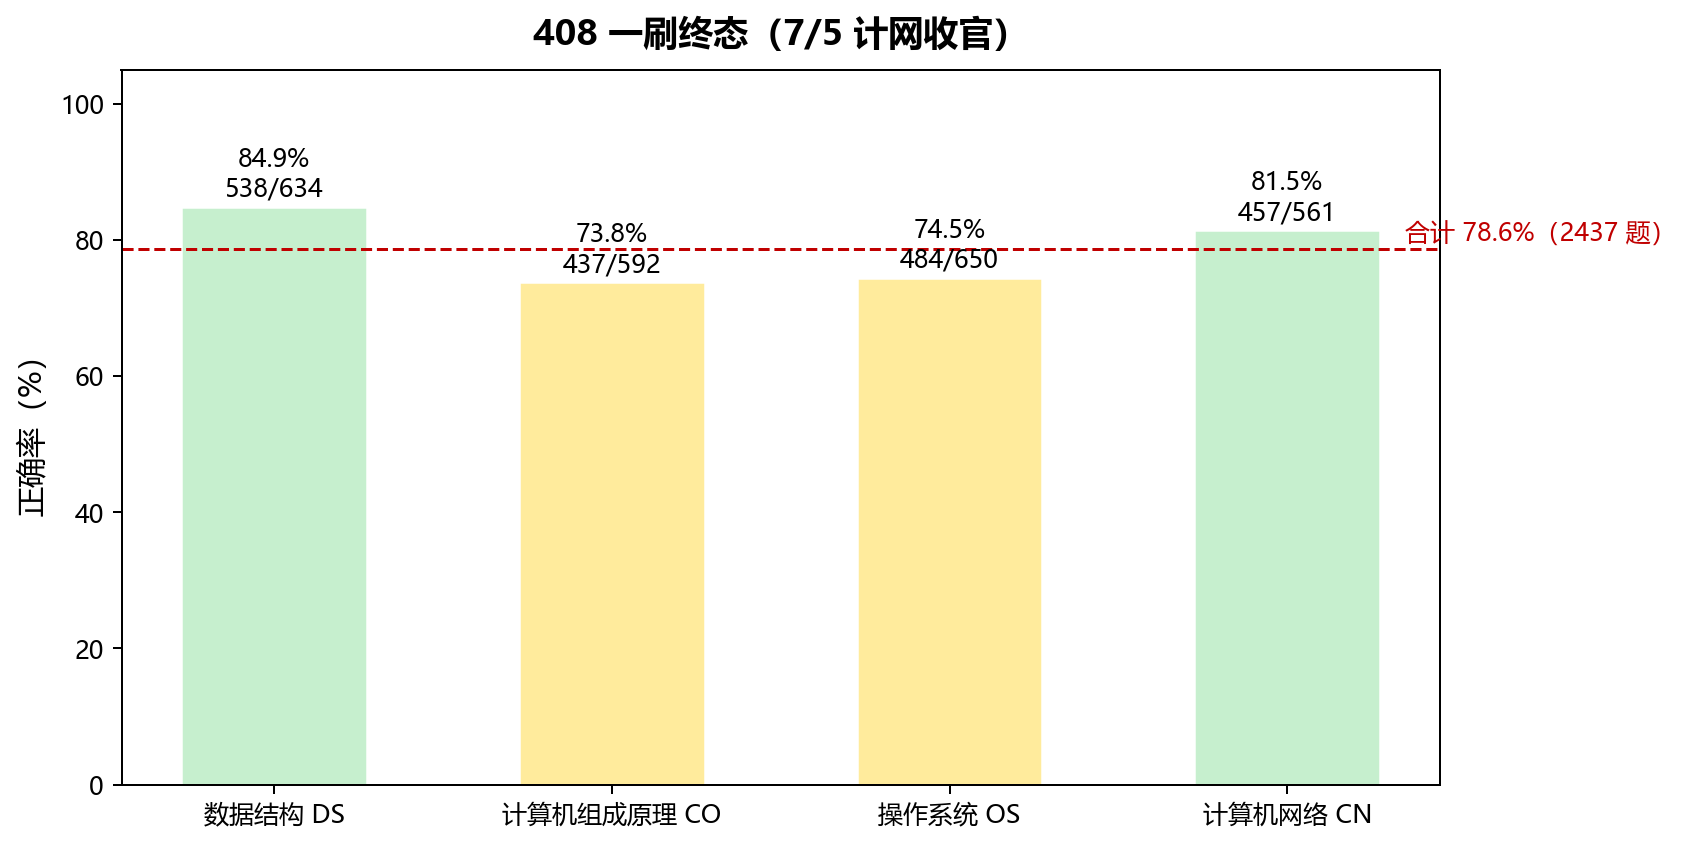
\includegraphics[width=0.8\textwidth]{july_408_final.png}
\caption{408 一刷终态（7/5 计网收官）}
\end{figure}

\textbf{状态提示}：408 一刷 7/5 收官后，7 月剩余时间没有再推进 408（与休息期重叠）。8 月需要启动二刷/真题专项，优先补强 CO I/O（真题 64.3\%）、OS 文件管理（真题 67.9\%）、DS 线性表（真题 50.0\%）。

\newpage

% ============================================================
\section{英语阅读（中断与恢复的完整证据）}
% ============================================================

\subsection{7 月逐篇明细}

\begin{table}[H]
\footnotesize
\centering
\begin{tabular}{llrrrr}
\hline
\rowcolor{headerbg}\textcolor{headerfg}{\textbf{年份/篇}} & \textcolor{headerfg}{\textbf{日期}} & \textcolor{headerfg}{\textbf{用时(分)}} & \textcolor{headerfg}{\textbf{正确/总}} & \textcolor{headerfg}{\textbf{正确率}} & \\
2017 Text 1 & 7/4 & 15 & 5/5 & 100\% & \\
2017 Text 2 & 7/7 & 19 & 4/5 & \cellcolor{greenrate}80\% & \\
2017 Text 3 & 7/8 & 12 & 4/5 & \cellcolor{greenrate}80\% & \\
2017 Text 4 & 7/9 & 19 & 3/5 & \cellcolor{yellowrate}60\% & \\
2018 Text 1 & 7/12 & 13 & 4/5 & \cellcolor{greenrate}80\% & \\
2018 Text 2 & 7/13 & 10 & 3/5 & \cellcolor{yellowrate}60\% & \\
2018 Text 3 & 7/16 & 16 & 4/5 & \cellcolor{greenrate}80\% & \\
2018 Text 4 & 7/17 & 17 & 4/5 & \cellcolor{greenrate}80\% & \\
2019 Text 1 & 7/18 & 16 & 5/5 & 100\% & \\
\rowcolor{yellowrate}7/19--7/26 & \multicolumn{4}{l}{休整约一周（无记录）} & \\
2019 Text 2 & 7/30 & 20 & 2/5 & \cellcolor{redrate}40\% & \\
2019 Text 3 & 7/31 & 14 & 5/5 & 100\% & \\
\rowcolor{grayrow}小计（11 篇；Text4 2019 未做） & & 15.5 平均 & 43/55 & 78.2\% & \\
\hline
\end{tabular}
\caption{英语阅读 7 月逐篇成绩（橙色行为休息期）}
\end{table}

\begin{figure}[H]
\centering
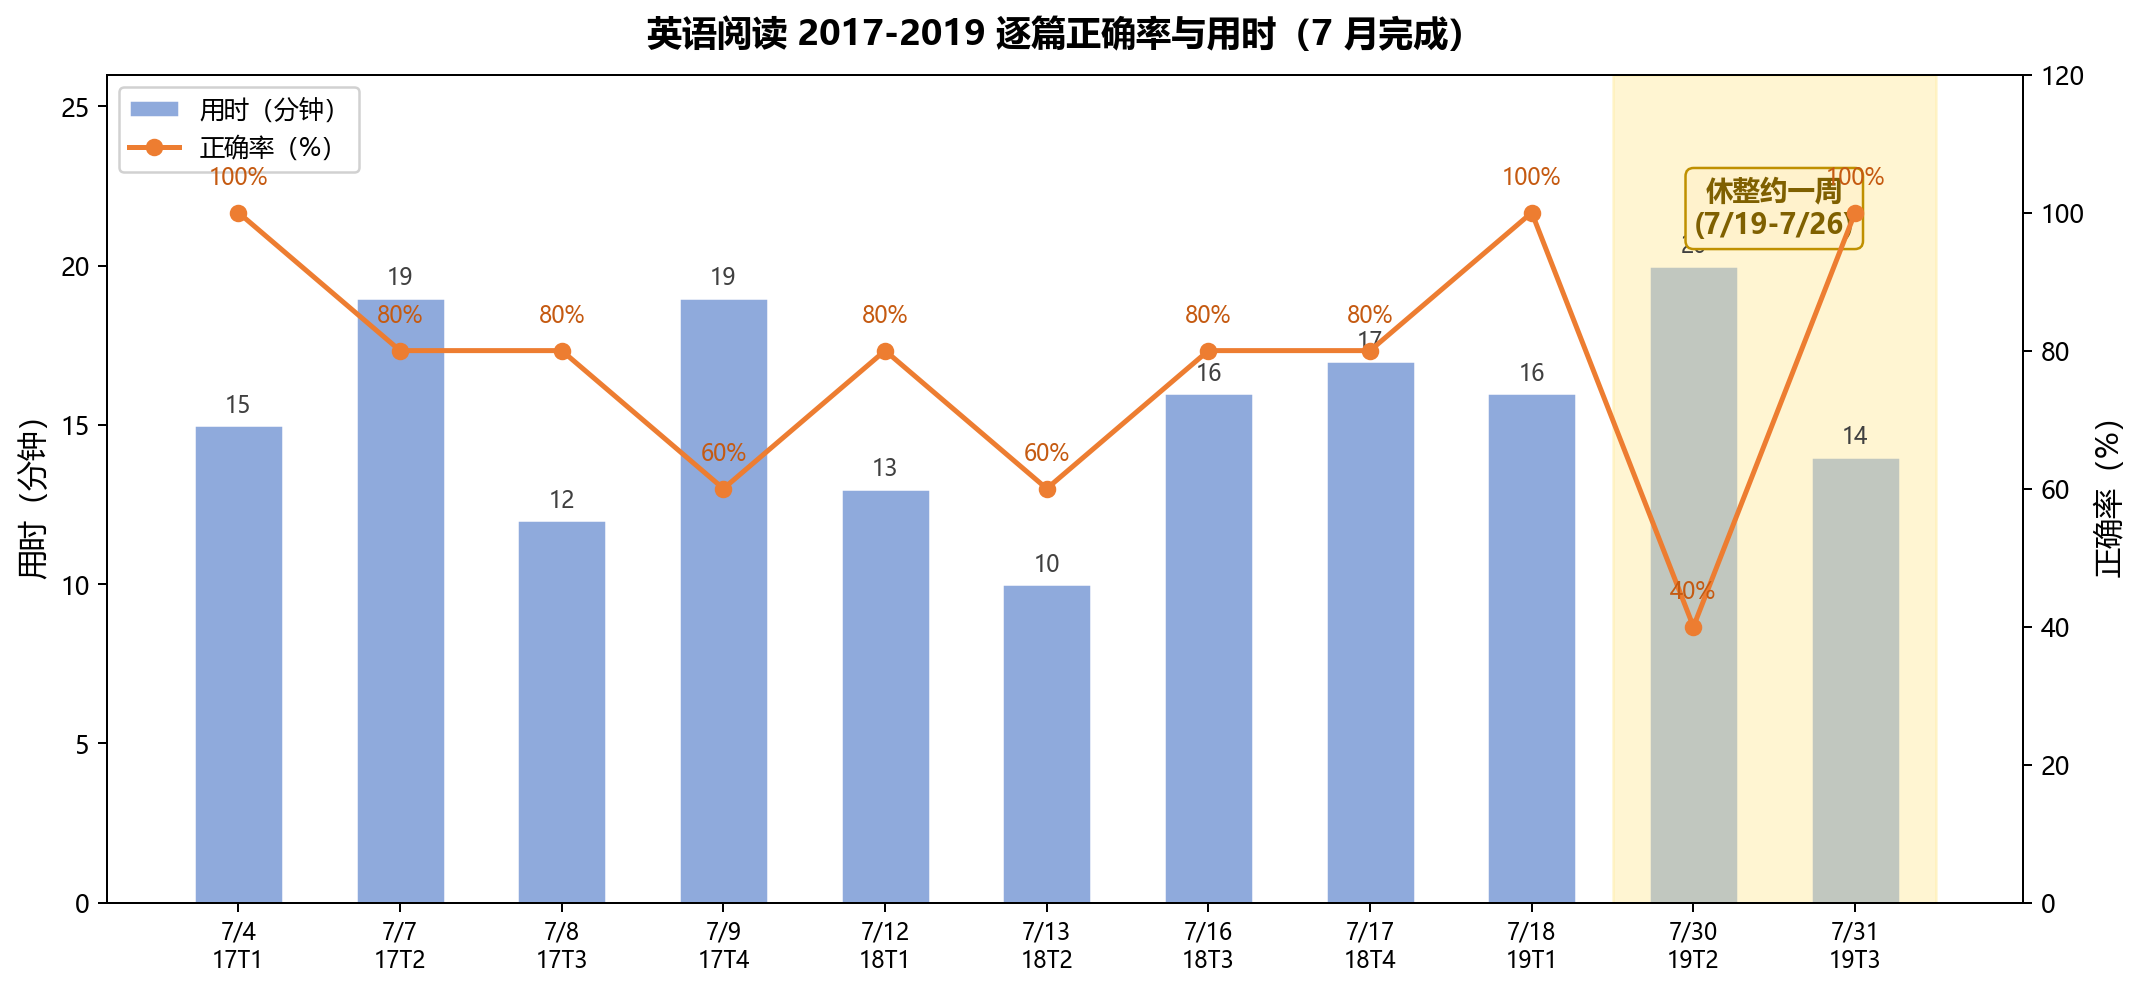
\includegraphics[width=0.95\textwidth]{july_english_break_recovery.png}
\caption{2017--2019 逐篇正确率与用时——黄色区域即休整期，恢复节奏一目了然}
\end{figure}

\subsection{阶段对比}

\begin{itemize}
\item \textbf{休整前}（7/4--7/18，9 篇）：平均 \textbf{15.2 分钟}，正确率 \textbf{80\%}。
\item \textbf{恢复初期}（7/30 一篇）：\textbf{20 分钟}（7 月最慢），正确率 \textbf{40\%}。
\item \textbf{恢复次日}（7/31 一篇）：\textbf{14 分钟}，正确率 \textbf{100\%}。
\end{itemize}

\subsection{累计状态}

\begin{itemize}
\item 2011--2019 已完成 \textbf{175 题 / 108 对 / 61.7\%}（按整卷口径含未做的 2019 Text4 计 0，为 180 题 / 60.0\%）。
\item 7 月完成的 2017--2019 三卷 \textbf{71.7\%}，明显高于 2011--2016 的 \textbf{54.2\%}——即使中断一周，恢复后的水平仍显著好于上半年，说明积累还在。
\item Text 4 是四篇中最弱的题型（已做 21/40 = 52.5\%）；2020--2026 共 140 题未做。
\end{itemize}

\begin{figure}[H]
\centering
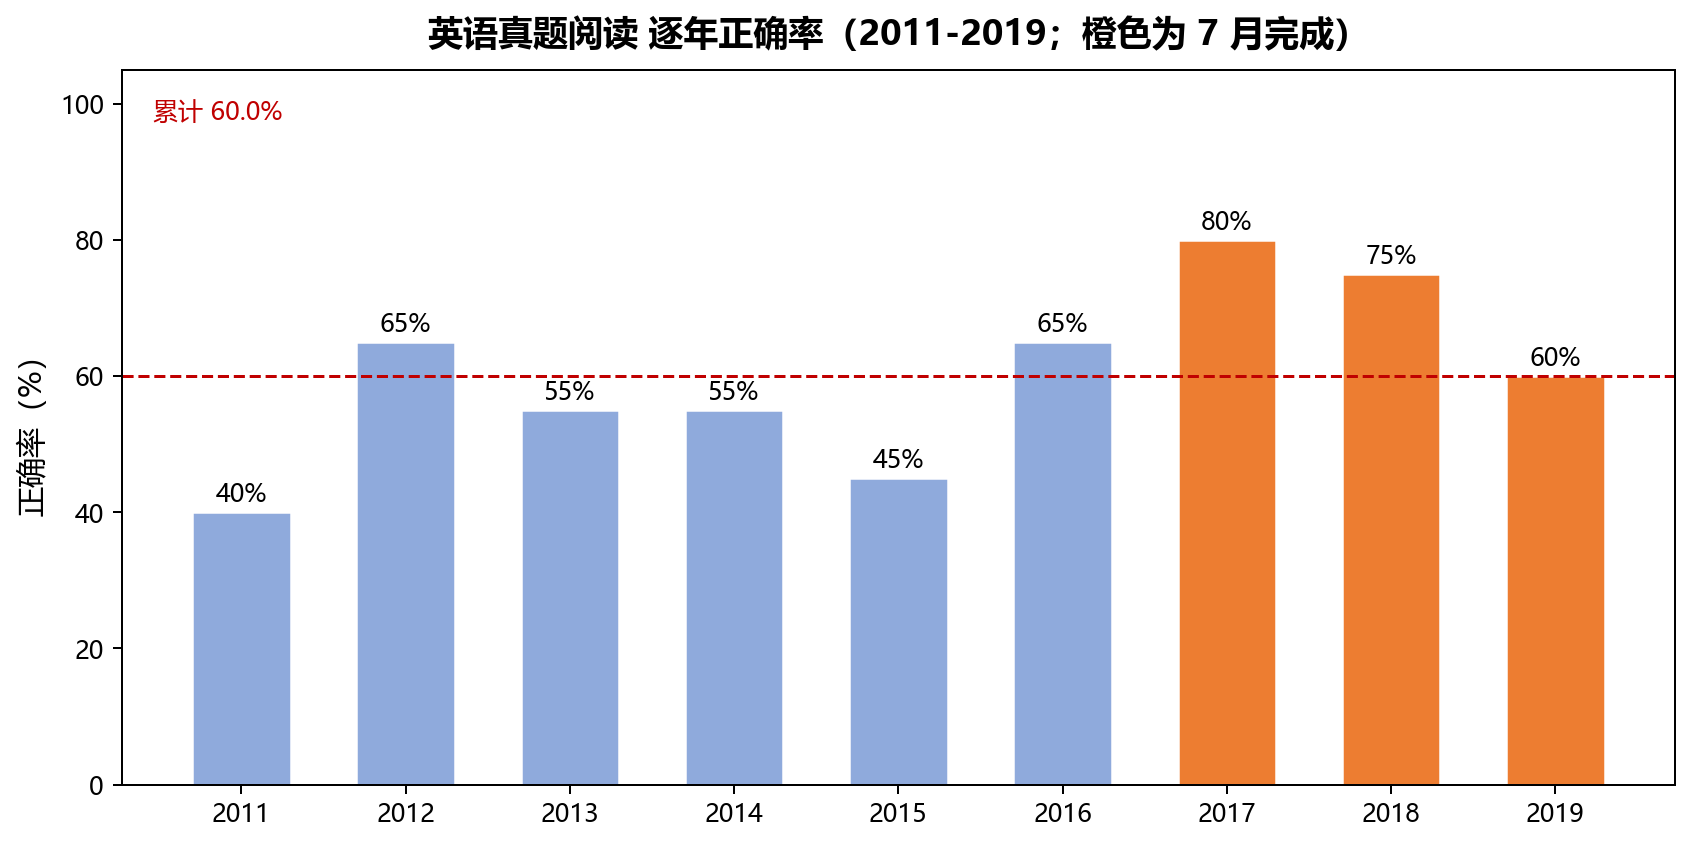
\includegraphics[width=0.8\textwidth]{july_english_yearly.png}
\caption{英语阅读逐年正确率（橙色为 7 月完成的 2017--2019）}
\end{figure}

\newpage

% ============================================================
\section{本月反思与下阶段重点}
% ============================================================

\begin{enumerate}[leftmargin=*,itemsep=6pt]
    \item \textbf{英语阅读仍是全局最短板}：累计正确率约 60\%，Text 4 最弱，且 2019 Text4、2020--2026 尚未完成。8 月建议恢复``隔天一篇 + 精读 + 墨墨真题词库''的节奏，把 2020--2026 补完。

    \item \textbf{数学解答/问答类题型偏弱}：严选题问答 69.2\%、880 解答 67.3\%，计算与步骤题的规范性问题要专门练；线代、概率、880 空间解析几何均未启动，强化进度需要提速。

    \item \textbf{408 需要重新捡起来}：一刷收官后停摆近一个月，建议 8 月上旬启动二刷/真题专项，优先级：CO I/O 系统、OS 文件管理、DS 线性表真题。

    \item \textbf{节奏管理的经验}：这次休息一周后，7/30 英语正确率 40\%、用时 20 分钟是``生疏期''的正常波动，7/31 就回到 100\%/14 分钟——短暂休息不会破坏积累，但要避免空窗超过一周，建议用``小步重启''（每天先固定 2--3 小时、固定时段）防止再次停摆。

\end{enumerate}

\end{document}
